\documentclass[a4paper,12pt]{article} % тип документа

% Поля страниц
\usepackage[left=2.5cm,right=2.5cm,
    top=2cm,bottom=2cm,bindingoffset=0cm]{geometry}
    
%Пакет дял таблиц   
\usepackage{multirow} 
    
%Отступ после заголовка    
\usepackage{indentfirst}


% Рисунки
\usepackage{floatrow,graphicx,calc}
\usepackage{wrapfig}

%%% Работа с картинками
\usepackage{graphicx}  % Для вставки рисунков
\graphicspath{{images/}{images2/}}  % папки с картинками
\setlength\fboxsep{3pt} % Отступ рамки \fbox{} от рисунка
\setlength\fboxrule{1pt} % Толщина линий рамки \fbox{}
\usepackage{wrapfig} % Обтекание рисунков и таблиц текстом

% Создаёем новый разделитель
\DeclareFloatSeparators{mysep}{\hspace{1cm}}

% Ссылки?
\usepackage{hyperref}
\usepackage[rgb]{xcolor}
\hypersetup{				% Гиперссылки
    colorlinks=true,       	% false: ссылки в рамках
	urlcolor=blue          % на URL
}


%  Русский язык
\usepackage[T2A]{fontenc}			% кодировка
\usepackage[utf8]{inputenc}			% кодировка исходного текста
\usepackage[english,russian]{babel}	% локализация и переносы


% Математика
\usepackage{amsmath,amsfonts,amssymb,amsthm,mathtools}

%%% Дополнительная работа с математикой
\usepackage{amsmath,amsfonts,amssymb,amsthm,mathtools} % AMS
\usepackage{icomma} % "Умная" запятая: $0,2$ --- число, $0, 2$ --- перечисление


% Что-то 
\usepackage{wasysym}


\begin{document}
\begin{center}
	\footnotesize{ФЕДЕРАЛЬНОЕ ГОСУДАРСТВЕННОЕ АВТОНОМНОЕ ОБРАЗОВАТЕЛЬНОЕ 			УЧРЕЖДЕНИЕ ВЫСШЕГО ОБРАЗОВАНИЯ}\\
	\footnotesize{МОСКОВСКИЙ ФИЗИКО-ТЕХНИЧЕСКИЙ ИНСТИТУТ\\(НАЦИОНАЛЬНЫЙ 			ИССЛЕДОВАТЕЛЬСКИЙ УНИВЕРСИТЕТ)}\\
	\footnotesize{ФАКУЛЬТЕТ ОБЩЕЙ И ПРИКЛАДНОЙ ФИЗИКИ\\}
	\hfill \break
	\hfill \break
	\hfill \break
	\hfill \break
    
\includegraphics[width=10cm,height=7cm,keepaspectratio]{mipt_eng_text_png.png}\\
    \hfill \break
	\hfill \break
	\hfill \break
	\hfill \break
	\large{Лабораторная работа № 2.5.1\\\textbf{Измерение коэффициента поверхностного натяжения жидкости}}\\
	\hfill \break
	\hfill \break
	\hfill \break
	\hfill \break
	\begin{flushright}
		Баранов Даниил\\
		Группа Б02-103
	\end{flushright}
	\hfill \break
	\hfill \break
	\hfill \break
\end{center}
\hfill \break
\hfill \break
\hfill \break
\hfill \break
\begin{center}
	Долгопрудный, 2022 г.
\end{center}
\thispagestyle{empty}
\newpage
	\textbf{Цель работы:} 1) измерение температурной зависимости  коэффициента поверхностного натяжения дистиллированной воды с использованием известного коэффициента поверхностного натяжения спирта; 2) определение полной поверхностной энергии  и теплоты, необходимой для изотермического образования единицы поверхности жидкости  при различной температуре.
	\hfill \break
	
	\textbf{В работе используются:} прибор  Ребиндера  с термостатом и микроманометром; исследуемые жидкости; стаканы.
	
\section{Теоретическая часть}
	Наличие поверхностного слоя приводит к различию давлений по разные стороны от искривленной границы раздела двух сред. Для сферического пузырька с воздухом  внутри жидкости избыточное давление даётся формулой Лапласа:
	\begin{equation}
		\label{laplas}
		\Delta P = \frac{2\sigma}{r},
	\end{equation}
	где $\sigma$ –- коэффициент поверхностного натяжения, $\Delta P$ – разница давлений внутри и снаружи пузырька, $r$ – радиус кривизны поверхности раздела двух фаз. Эта формула лежит в основе предлагаемого метода определения коэффициента поверхностного натяжения жидкости.
\section{Экспериментальная установка}
	Исследуемая жидкость (дистиллированная вода) наливается в сосуд (колбу) \textbf{В} (рис.~\ref{ris:ustanovka}). Тестовая жидкость  (этиловый спирт) наливается  в сосуд \textbf{E}. При измерениях  колбы герметично закрываются  пробками.   Через одну из двух пробок  проходит полая металлическая игла \textbf{C}. Этой пробкой закрывается сосуд, в котором  проводятся измерения. Верхний конец иглы открыт в атмосферу, а нижний погружен в жидкость. Другой сосуд герметично закрывается второй пробкой. При создании достаточного  разряжения воздуха в колбе с иглой пузырьки воздуха начинают пробулькивать через жидкость. Поверхностное натяжение можно определить по величине разряжения $\Delta P$ (\ref{laplas}), необходимого для прохождения пузырьков (при известном радиусе иглы).\\
	Разряжение в системе создается с помощью аспиратора \textbf{A}. Кран \textbf{K2} разделяет две полости аспиратора. Верхняя полость при закрытом кране \textbf{K2}  заполняется водой. Затем кран \textbf{K2} открывают и заполняют водой  нижнюю полость  аспиратора.  Разряжение воздуха создается в нижней полости  при открывании крана \textbf{K1}, когда  вода вытекает из неё по каплям. В колбах \textbf{B} и \textbf{C}, соединённых трубками с нижней полостью аспиратора,  создается такое же пониженное давление. Разность давлений в полостях с разряженным воздухом и атмосферой измеряется спиртовым микроманометром.
	\begin{figure}[H]
		\center{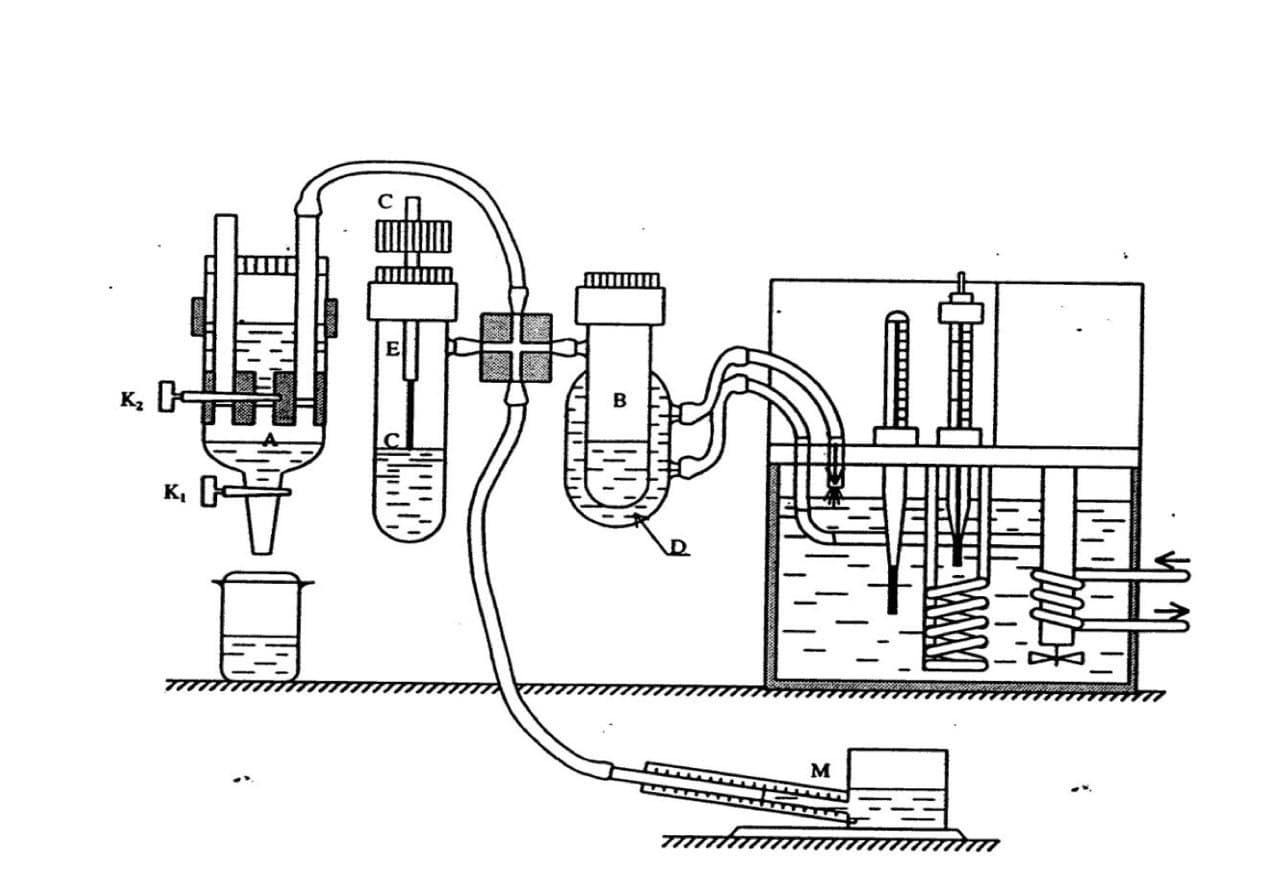
\includegraphics[width=12cm,height=12cm,keepaspectratio]{установка.jpg}}
		\caption{Схема установки для измерения температурной зависимости коэффициента поверхностного натяжения.}
		\label{ris:ustanovka}
	\end{figure}
\section{Экспериментальные данные}
	В таблице~\ref{table:const} приведены константы, используемые в лабораторной работе. 	
\floatsetup[table]{capposition=top}	
\begin{table}[H]
	\caption{Постоянные величины.}
	\label{table:const}
\begin{tabular}{|c|c|c|c|c|}
	\hline
	\begin{tabular}[c]{@{}c@{}}Плотность\\ этанола\\ $\rho_0$, кг/м$^3$\end{tabular} & \begin{tabular}[c]{@{}c@{}}Плотность\\ воды\\ $\rho$, кг/м$^3$\end{tabular} & \begin{tabular}[c]{@{}c@{}}Ускорение\\ свободного \\ падения\\ $g$, м/c$^2$\end{tabular} & \begin{tabular}[c]{@{}c@{}}Пересчетный\\ коэффициент\\ $k$\end{tabular} & \begin{tabular}[c]{@{}c@{}}Коэффициент\\ поверхностного натяжения\\ этанола (T = 20$^\circ$С)\\ $\sigma_0$, мН/м\end{tabular} \\ \hline
	809,5 & 1000,0 & 9,81 & 0,2 & 22,75                                                                                                                         \\ \hline
\end{tabular}
\end{table}


	В таблице~\ref{table:error} приведены значения и случайные ошибки измерения величин, определяемых в ходе эксперимента.
\floatsetup[table]{capposition=top}	
\begin{table}[H]
	\caption{Некоторые величины и их погрешность.}
	\label{table:error}
\begin{tabular}{|c|c|c|c|}
	\hline
	& \begin{tabular}[c]{@{}c@{}}Температура\\ $T$, К\end{tabular} & \begin{tabular}[c]{@{}c@{}}Длина столба спирта\\ в микроманометре\\ $h$, мм\end{tabular} & \begin{tabular}[c]{@{}c@{}}Пересчитанные показания\\ микроманометра\\ $P$, Па\end{tabular} \\ \hline
	Величина  & 294,5   & 175,0  & 277,9 \\ \hline
	Погрешность & 0,2 & 0,5 & 0,8 \\ \hline
	$\varepsilon$, \% & 0,03 & 0,3 & 0,3 \\ \hline
\end{tabular}
\end{table}


	Результаты измерений радиуса иглы приведены в таблице~\ref{table:radius}. Для проверки достоверности полученного результата диаметр иглы был измерен дополнительно на микроскопе: $d = 1,05 \pm 0,02$ мм.
\floatsetup[table]{capposition=top}	
\begin{table}[H]
	\caption{Радиус используемой иглы.}
	\label{table:radius}
\begin{tabular}{|c|c|c|c|c|c|}
	\hline
	$T$, $^\circ$C & $h$, мм & $\Delta P$, Па & $r$, мм & $\sigma_r$, мм & $\sigma_r / r$, \% \\ \hline
	21,4 & 41 & 80,4 & 0,56 & 0,008 & 1,4 \\ \hline
\end{tabular}
\end{table}	


	В таблице~\ref{table:main} приведены результаты измерений, позволяющих исследовать зависимость $\sigma = \sigma (T)$.
\floatsetup[table]{capposition=top}	
\begin{table}[H]
	\caption{Результаты измерений.}
	\label{table:main}
\begin{tabular}{|c|c|c|c|c|c|}
	\hline
	$T$, $^\circ$C & $h$, мм & $\Delta P$, Па & $\sigma$, мН/м & $\sigma_\sigma$, мН/м & $\sigma_\sigma / \sigma$, \% \\ \hline
	21,4           & 231,0   & 257,0          & 66,8           & 1,5                   & 2,3                          \\ \hline
	25,4           & 230,0   & 255,3          & 66,4           & 1,5                   & 2,3                          \\ \hline
	30,3           & 228,0   & 251,3          & 65,3           & 1,5                   & 2,3                          \\ \hline
	35,2           & 227,0   & 249,4          & 64,8           & 1,5                   & 2,3                          \\ \hline
	39,9           & 226,0   & 247,4          & 64,3           & 1,5                   & 2,3                          \\ \hline
	45,0           & 224,0   & 243,5          & 63,3           & 1,5                   & 2,3                          \\ \hline
	49,9           & 222,5   & 240,5          & 62,5           & 1,5                   & 2,3                          \\ \hline
	54,9           & 219,0   & 233,7          & 60,8           & 1,5                   & 2,3                          \\ \hline
	59,8           & 218,0   & 231,7          & 60,2           & 1,5                   & 2,3                          \\ \hline
\end{tabular}
\end{table}


	По полученным данным построим график зависимости $\sigma = \sigma (T)$ (рис.~\ref{ris:Graph_1}) и проанализируем его (\ref{table:Graph_1}).
	\begin{figure}[H]
		\center{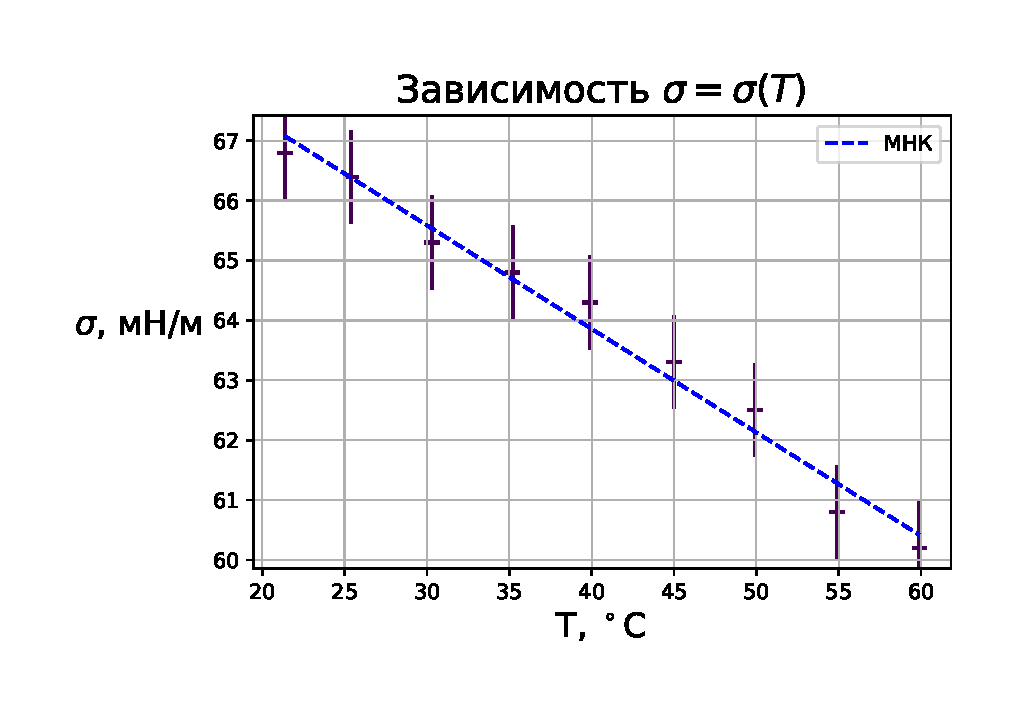
\includegraphics[width=450]{sigma.pdf}}
		
		\caption{Зависимость $\sigma = \sigma (T)$.}
		\label{ris:Graph_1}
	\end{figure}


\floatsetup[table]{capposition=top}	
\begin{table}[H]
	\caption{Анализ зависимости $\sigma = \sigma (T)$.}
	\label{table:Graph_1}
\begin{tabular}{|c|c|c|}
	\hline
	$d\sigma / d T$, мН/м$\cdot^\circ$C & Погрешность, мН/м$\cdot^\circ$C & $\epsilon$, \% \\ \hline
	-0,17                               & 0,01                            & 5,9            \\ \hline
\end{tabular}
\end{table}


	Дополнительно найдем зависимость теплоты образования единицы поверхности жидкости $q =~-T\frac{d\sigma}{dT}$ и поверхностной энергии единицы площади $U/\Pi =~\sigma + q$ от температуры. Результаты вычислений представлены в таблице~\ref{table:Graph_2-3}, а графики на рис.~\ref{fig:Graph_2} и рис.~\ref{fig:Graph_3}.
	\floatsetup[table]{capposition=top}	
	\begin{table}[H]
		\caption{Результаты дополнительных вычислений.}
		\label{table:Graph_2-3}
\begin{tabular}{|c|c|c|c|c|c|c|c|c|c|}
\hline
$T$, К        & 294,4 & 298,4 & 303,3 & 308,2 & 312,9 & 318 & 322,9 & 327,9 & 332,8 \\ \hline
$q$, мДж/м$^2$     & 50  & 51    & 52    & 52    & 53    & 54  & 55  & 56  & 57  \\ \hline
$U/\Pi$, мДж/м$^2$ & 116,8 & 117,4   & 117,3   & 116,8   & 117,3   & 117,3 & 117,5 & 116,8 & 117,2 \\ \hline
\end{tabular}
	\end{table}
	
	
	\thisfloatsetup{floatrowsep=mysep}	
	\begin{figure}[h!]
		\begin{floatrow}
			\ffigbox[\FBwidth]{\caption{Зависимость $q = q(T)$.}\label{fig:Graph_2}}%
			{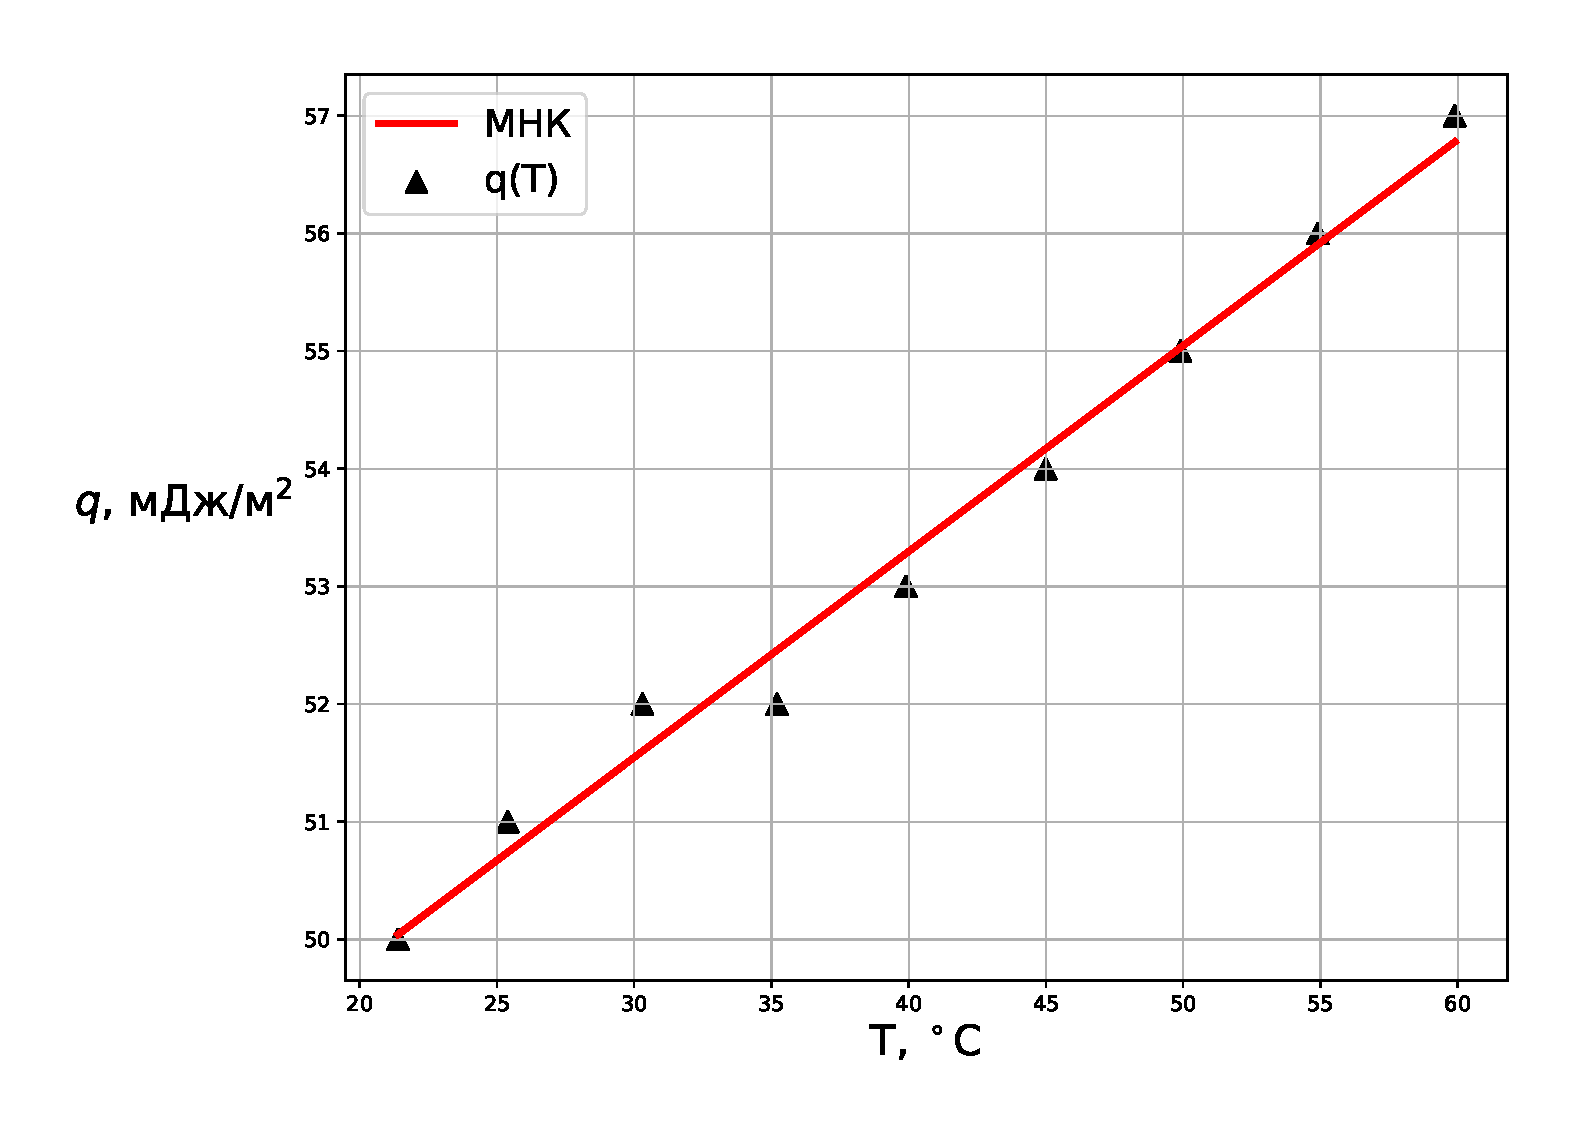
\includegraphics[width=15cm]{q.pdf}}
		\end{floatrow}
	\end{figure}
	
	\begin{figure}[h!]
		\begin{floatrow}
        	\ffigbox[\FBwidth]{\caption{Зависимость $U/\Pi$ от $T$.}\label{fig:Graph_3}}%
        			{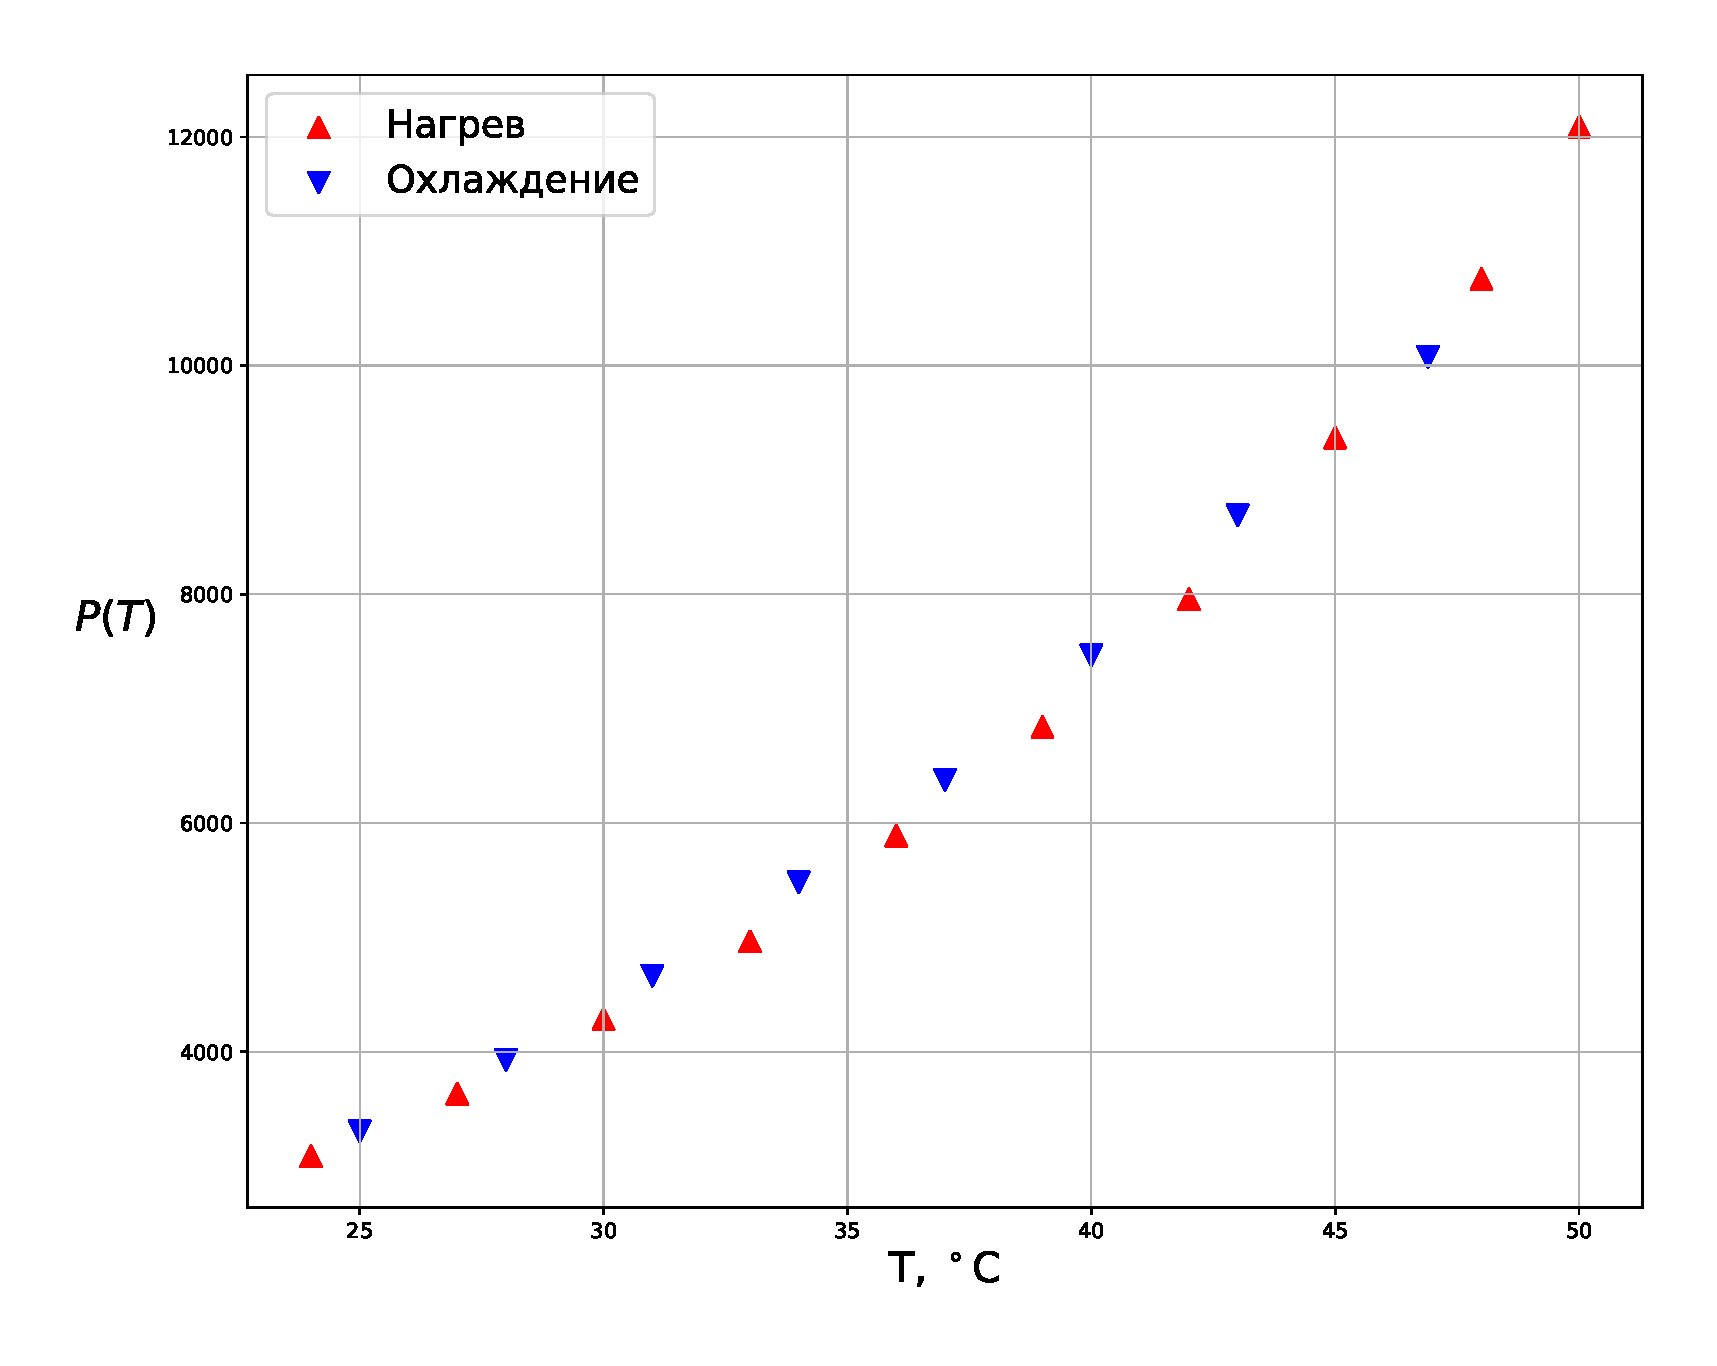
\includegraphics[width=15cm]{ener.pdf}}
        \end{floatrow}
	\end{figure}

\newpage
\section*{Обсуждение полученных результатов}
\begin{itemize}
	\item 
		В интервале температур от 23$^\circ$C до 60$^\circ$C зависимость $\sigma = \sigma(T)$ является линейной с коэффициентом наклона $d\sigma / dT = (-0,17\,\pm\, 0,01)$  мН/м$\cdot^\circ$C.Стоит отметить, что наш результат в пределах погрешности совпадает с табличным значением $d\sigma / dT \approx -0,16$.
	\item 
		Теплоты образования единицы поверхности жидкости $q = q(T)$ линейно зависит от температуры на исследуемом интервале температур.
	\item 	
		Внутренняя энергия поверхности $U/\Pi$ не зависит от температуры и есть константа $U = 117$ мДж/м$^2$.
\end{itemize}	
\end{document}
